\chapter{Exploring the preference of walking duration to rail transit stations by individual attributes}
\markright{CHAPTER 2}

% 待修正
\section{Introduction}
% walking access 在决定乘客量上的重要性

% 解释walking access和catchment area的关系,并说明目前的catchment area都是如何
% 明确不同属性的人具有不同的出行时间偏好
% 尽管明确有偏好,还要再明确目前已有研究没有得到出行者属性与步行时间偏好的定量关系
% 给出本研究的purpose和organization


% 略微重复一点第一章内容,说明我要做的背景.
% 步行很重要
% 步行是决定公交使用的重要因素
\subsection{Background}
Walking is the most important way to reach a transit station, people choose to take transit only when the walking access is within the acceptable range. People’s willingness to walk to transit has largely defined the catchment area of a station. This catchment area determined the population served by that station, for which it is also widely accepted as a key system performance measure of the transit station \cite{fielding1978performance,el2014new,chia2016walking}. 

% 好多针对步行的研究。
Walking access, either distance or duration, has been paid extensive attention to determine the catchment area of stations. However, delineating this area is a complex issue as the catchment area varies due to the different transit types and people's walking preferences. At present, the 800 meters (half-mile) transit catchment area, whether radial-based or road-network-based, has been widely accepted as a principal reference to the catchment area around rail transit stations \cite{kuby2004factors,gutierrez2011transit,cardozo2012application,zhao2013influences}, and a 400 meters (quarter-mile) catchment area is commonly defined around bus stops \cite{o1992analysis,zhao2003forecasting}. On the other hand, researchers also used some other catchment areas due to different research purposes and research contents. For example, a relatively small area of 250-meter buffer was adopted to analyzing the quality of access to the BRT stop
\cite{estupinan2008relationship}; a 500-meter buffer area was used in finding the factors generating boarding at metro stations in Seoul. Korea \cite{sohn2010factors}. Jun et al. segmented the catchment area into the core area, primary area, and secondary area, corresponding to 300 meters, 600 meters, and 900 meters pedestrian area respectively \cite{jun2015land}.

\subsection{Statement of problem}
% 说catchment area都是基于步行时间的,然后说明目前通用的
The most widely used 400-meter or 800-meter catchment area is commonly obtained from the sampling survey by loosely asking how far or how long people are willing to walk to rail transit stations, and the same reasoning has been used to justify other rail transit catchment areas and even in different cities and countries. These simplified catchment areas were applied to all the transit stations ignoring the differences in stations and the passengers, obviously, this "one size fits all" solution to catchment area should not be effective \cite{zhao2003forecasting,chia2016walking}. As to passengers, the acceptable walking access should not only relate to the station types, but also affected by the walking preference of passengers. Walking preferences, however, vary by destination, trip purpose, gender, age, land-use, safety, weather, and the price and availability of parking. 

% 步行偏好已经被确认,但关系没有明确
Various factors belong to the individual attributes pertaining to walking access have been attempted and confirmed in the literature, such as trip purpose, income level, occupation etc. \cite{alshalalfah2007case, weinstein2008far,chia2016walking}. However, little is known about the quantitative relationship between walking access and individual attributes, studies based on statistical description take account the majority. Even though some studies attempted regression approach to estimate the influence of individual attributes on the walking access, very little obtained a significant result \cite{jiang2012walk,daniels2013explaining}. It seems that the linear relationship between waking access and individual attributes does not exist.

\subsection{Research purpose and contents}
% 提出目的,对象,章节组织
% Introduction的总结
This study aims to explore the quantitative relationship between walking access and individual attributes and try to predict the walking preference of accessing transit stations using individual attributes. The study case used in this study is the rail transit passengers of Fukuoka City, Japan. The contents of this study are organized as follows: section two reviews the previous research on the walking access to transit station, based on which the research questions are put forward; section three interprets the methodology; section four gives the descriptions of data; section five shows the process and results of analysis; section six discusses the results and draws the conclusion. 

%
\section{Literature review}
% 对目前的walking access研究整理
% 对walking access的解释
% 影响因素
% 给出本研究的研究假设,研究对象,研究思路。

In the studies of walking access, there is always a difficult point in obtaining the accuracy walking duration/distance by questionnaire because of the discrepancy between perceived values and objective values. Also, the observed walking duration/distance is not the reflection of acceptable range of walking access, but just the walking duration/distance between departures and stations. For this problem, some studies chose a different perspective to explain the walking access by introducing a threshold of walking duration \cite{besser2005walking,mccormack2008objective}. They examined the differences in the distribution of influencing factors in terms of the specific threshold of walking duration. Indeed, using a threshold can decrease the discrepancy between observation and reality in some extent, but this disposal also brought some new problems in, for example, it may lead to a great loss of information in the raw data, and it is also difficult to decide the threshold of walking duration.

%
Another point of this issue is whether using the walking distance or walking duration as the research object. To date, there are a lot of studies working on the relationship between walking access and individual attributes, some of them argued that an individual has a limited amount of time spending on traveling in one day. People with faster walking speed tend to accept a further walking distance  \cite{marchetti1994anthropological,larsen2010beyond}. With this reasoning it is easy to think of that passengers with the same individual attributes may have the similar willingness of walking duration, but they generally have different willingness of walking distance due to different travel speed.

%
Among the influencing factors of walking access, individual attributes are generally thought to be the key that can affect walking distance \cite{besser2005walking,weinstein2008far,krygsman2004multimodal,yang2012walking,daniels2013explaining,guerra2012half}, whereas, little literature has clearly verified the quantitative relationship between individual attributes and walking access, even there is a study suggesting the walking distance should not be viewed as a function of individual attributes \cite{krygsman2004multimodal}. Several studies have confirmed the role of travel purposes in determining walking distance, the commute trips showed particularity from the other purposes. People who have the travel purpose of commute tend to accept a longer walking access to rail transit stations \cite{larsen2010beyond}. However, the definite relationship between trip purposes and walking distance is still unclear. The situation is the same with other categories of factors, such as the factors of transportation environment, land-use, and willingness of passengers \cite{guerra2012half,krygsman2004multimodal,weinstein2008far}. The only thing that has been confirmed to date is that the walking access can be influenced by some specific kinds of factors, such as socio-demographic characteristics, trip purposes, and built-environment, but the problem is how the walking access is influenced by those factors. 

% Summary
As interpreted above, the walking access is a just direct reflection of the distance between departures and stations, which should not have a direct relationship to individual attributes. Some studies attempting regression model to deal with this problem also supported this argument that no significant quantitative relationship was found between walking access and individual attributes. However, the results from extensive studies working on the qualitative description of the walking distance distribution have clearly shown that individual attributes have an impact on the walking access to rail transit stations. It is supposed that it may due to some inappropriate understanding of the surveyed walking access, and inappropriate assumption of the relationship form between individual attributes and walking access. Focusing on the probable inadequacies summarized from the previous studies, the flow of the research process is organized as Figure \ref{fig:chp2:Chp2Flowchart}.

% Figure 1
\begin{sidewaysfigure}[htbp]
	\centering
	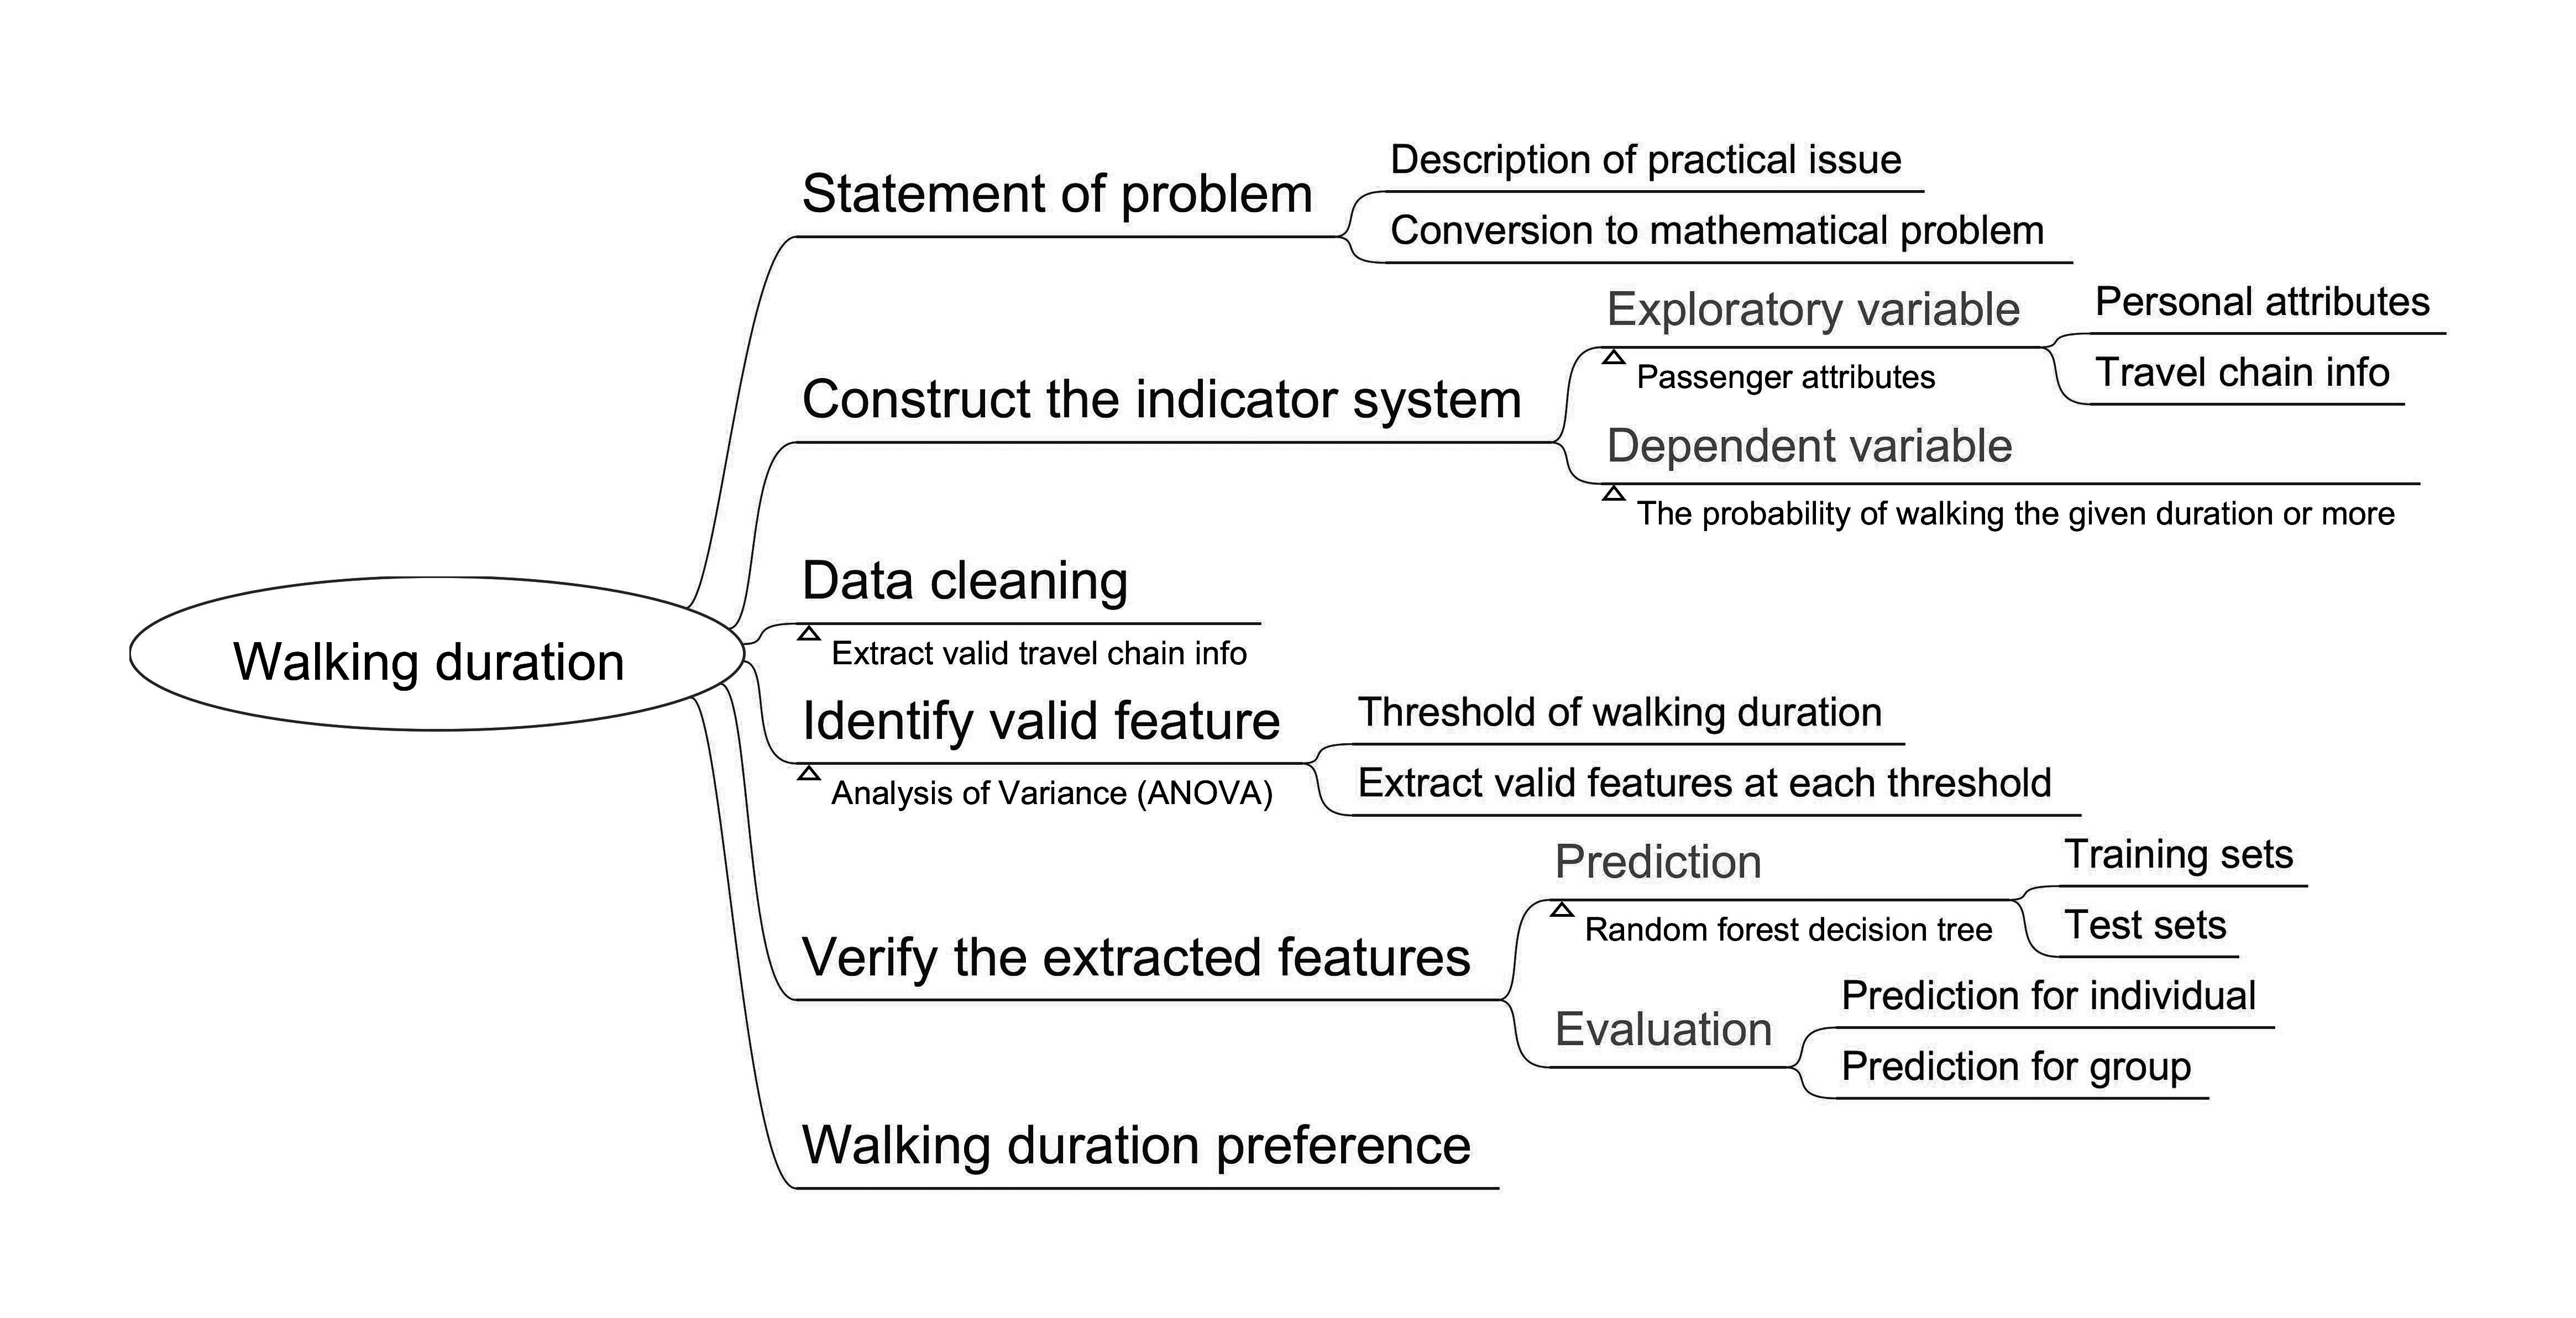
\includegraphics[width=\linewidth]{chapter2/BWChp2Flowchart}
	\caption{Research flowchart}
	\label{fig:chp2:Chp2Flowchart}
\end{sidewaysfigure}

%
\section{Methodology}
% 现实问题描述。1. PPT部分的描述。2. 把现在introduction中的类比部分拿过来
% 问题转换。1. Introduction部分的描述。2. PPT部分的描述。3. Feature estimation部分的抽象模型拿过来
% PPT上假设的图搬过来。最后要给出一个总结

\subsection{Description of realistic problem}
% 一个类比
Rail transit provides a cheaper and environment-friendly way of transportation to passengers. Like any other service and commodities, it needs to face the market and to be transacted at the price acceptable to consumers. This accepted transaction price means that any price cheaper than that can be accepted by the consumers. As a result, consumers with various consumption-ability will have different characteristics distribution of any specific transaction price. Obviously, the same for rail transit users. For the operator of rail transit, it is important to know how much the cost that consumers are willing to pay, based on which thereby making rail transit more attractive. But unlike the general service and commodities, the cost refers more to the convenience but not the fare for passengers. Because the cheap enough fare is already not an important element for passengers to decide whether using rail transit, while the walking access to stations has become an important determinant.

% 转换回轨道交通乘客时的选择问题
For the issue of riding rail transit, before a potential passenger makes the decision on walking to a station, the walking access, which is the "price" for this potential passenger, is just the reflection of the distance between departures and stations. In case this walking access is accepted by this potential passenger, this trip will happen and it can be surveyed. Based on the analogy given above, it's easy to think of that passengers with different individual attributes should have different willingness towards walking access to stations, and the surveyed walking access can be viewed as the transaction price which has been accepted by passengers. It follows that a less walking access will lead to an increase in the willingness of using rail transit, which reflected on the survey data will be that the records of shorter walking duration are more than that of longer walking duration. 

% 数学描述
\subsection{Conversion to mathematical problem}
% 重申研究对象,dependent variable,independent variables,提出抽象模型
The study aims to find the relationship between surveyed waking duration and passenger attributes. Based on the above comparison between the behaviors of using transit and consumption, it can be concluded that passenger attributes have an impact on the willingness of walking duration, but not on the surveyed walking duration. The abstract functional relationship between walking duration and passenger attributes is given in \ref{eq:chp2:AbstractFunction}. This abstract function indicates that we need to find the expression of walking duration to describe the passenger willingness, also to find out the functional relationship between the walking duration expression and passenger attributes.

% equation
\begin{equation}
Expression(Walking\ duration) = Function({factor}_1, {factor}_2, {factor}_3, \ldots)
\label{eq:chp2:AbstractFunction}
\end{equation}

% 提出用threshold,并结合上边提到的消费能力,给出数学描述,转化为binary choice
From the perspective of consumption-ability interpreted before, if giving a specific threshold of walking duration, the probability of accepting this threshold will vary due to different passenger attributes. Based on the interpretation, this mathematical problem can be converted into that to examine the impact of passenger attributes on the probability of accepting a given threshold of walking duration. The model can be expressed as follows: Equation \ref{eq:chp2:threshold} gives the expression of walking duration describing the passenger willingness by $Y^T_i$, and Equation \ref{eq:chp2:probability} is the function of this willingness and passenger attributes that the probability of walking the threshold $T$ or more in terms of the passenger attributes of $X_i$.

% & 符号为对齐符号,用于 table 或 matrix
\begin{equation}
\left\{\begin{matrix}
Y^T_i=1,&(t_i>T) \\
Y^T_i=0,&(t_i<T)
\end{matrix}\right.
\label{eq:chp2:threshold}
\end{equation}

\begin{equation}
P(Y^T_i=1 \mid X_i)=F(X_i)
\label{eq:chp2:probability}
\end{equation}

%
\begin{enumerate}
	\setlength{\parskip}{0\baselineskip} % 设置段间距
	\normalsize
	\item[\textbf{Where:}]
	\item[$t_i$] is the walking duration answered by passenger $i$ (in minutes).
	\item[$T$] is the threshold of walking duration that to be examined (in minutes).
	\item[$Y^T_i$] is a binary variable. $Y^T_i=1$ means passenger $i$ walked a longer walking duration than the threshold of $T$; while $Y^T_i=0$ means walked less than the threshold.
	\item[$X_i$] is the vector whose component is the individual attributes passengers.
	\setlength{\parskip}{0.7\baselineskip} % 设置段间距
\end{enumerate}


% 提出假设
\subsection{Basic hypothesis}
% 一个简短说明,为什么要假设
A large number of existing studies have shown that passenger attributes can affect walking access to rail transit station. Combining with the statement of problem conversion, this study proposes the first basic hypothesis that, passengers with different attributes have distinct walking behavior to access rail transit. In addition, since walking access is the direct reflection of the distance between transit stations and departures, the distribution of passengers' departures also affects the walking access to transit. The second hypothesis aims to simplify this problem by ignoring the distribution of passengers' departures, thus focusing on the influence of passenger attributes to the walking access. Moreover, since the dependent variable in this study is converted in to the probability of accepting the given threshold of walking duration, the third hypothesis is proposed to ensure the answered walking duration is an accepted one. The specific definitions of the hypothesis are as follows.

\begin{itemize}
	\setlength{\parskip}{0\baselineskip} % 设置段间距
	\item H1: The willingness of walking duration of people with the same attributes should subject to the normal distribution.
	\item H2: The departures and destinations of people with different attributes in Fukuoka are randomly distributed.
	\item H3: The respondents are viewed as they can accept the walking duration that they answered.
	\setlength{\parskip}{0.7\baselineskip} % 设置段间距
\end{itemize}

According to the H1 and H2, if considering the walking duration $T$, set the proportion of $k$ group in the whole surveyed sample as $r_k$. The proportion of passengers walking less than the given threshold $T$ is marked as $r_{k}^{<T}$, while the proportion of passengers walking more than the given threshold $T$ is marked as $r_{k}^{>T}$. If passenger attributes have no significant correlation to the accepted walking duration, then the three index $r_k$, $r_{k}^{<T}$ and $r_{k}^{>T}$ will not show significant differences. Otherwise, the three proportion should show significant differences, and the differences will show regularities at different threshold $T$. Figure \ref{fig:chp2:Chp2HypothesisOfWalkingDurationDistribution} shows the expected differences in the distribution of investigated walking duration in terms of passengers with different attributes. 

Based on H3, if someone gives the answer $t$ minutes, it means this respondent can accept the walking duration of $t$ minutes and any walking duration that less than $t$ minutes. Indeed, this respondent perhaps can accept the walking duration longer than that he answered, but this study just concerns about if he can accept the given threshold of the walking duration other than how long he can accept.

% 要给出这个图的说明
\begin{figure}[htbp]
	\centering
	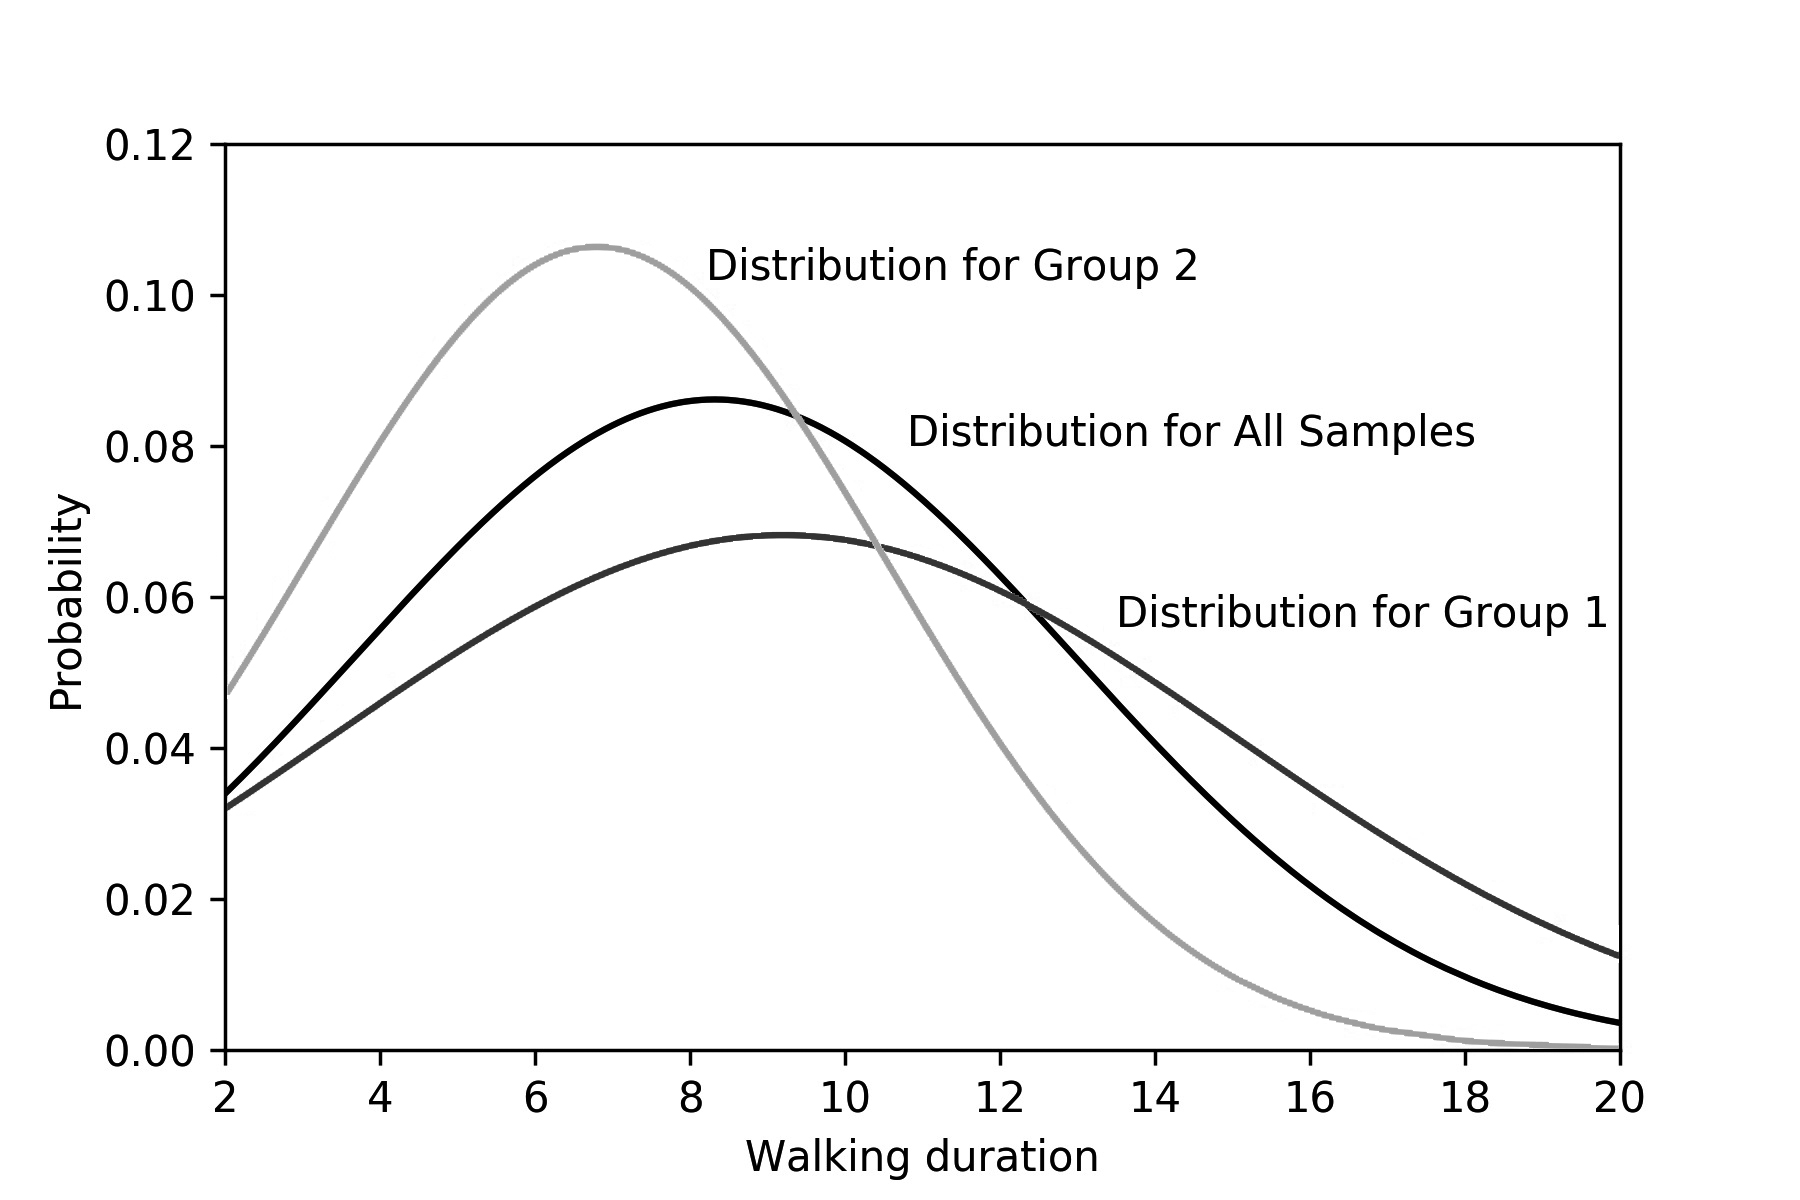
\includegraphics[width=\linewidth]{chapter2/HypothesisDistribution}
	\caption{Hypothesis of walking duration distribution}
	\label{fig:chp2:Chp2HypothesisOfWalkingDurationDistribution}
\end{figure}

%
\section{Data}
%
\subsection{Case introduction}
The research case of this study is Fukuoka, Japan. All the rail transit stations and rail transit passengers within the urban area of Fukuoka are investigated as the research objects. The data set is extracted from the Northern Kyushu Area Person Trip Survey, which is conducted about every 12 year, the latest available data is from the 4th survey surveyed by the year of 2005, and the 5th survey is already in preparation from September 2017. Figure \ref{fig:chp2:StationDistribution} shows the research area and the distribution of rail transit stations. By the year of 2005 (the 4th Northern Kyushu Area Person Trip Survey was conducted), there are more than 70 stations located within the city area of Fukuoka, of which the number of JR Kyushu station is 27, Fukuoka Subway station is 35, and West Japan Railway station is 16. Now some new rail transit lines and stations are still under planning and construction. 

% Figure 1
\begin{figure}[htbp]
	\centering
	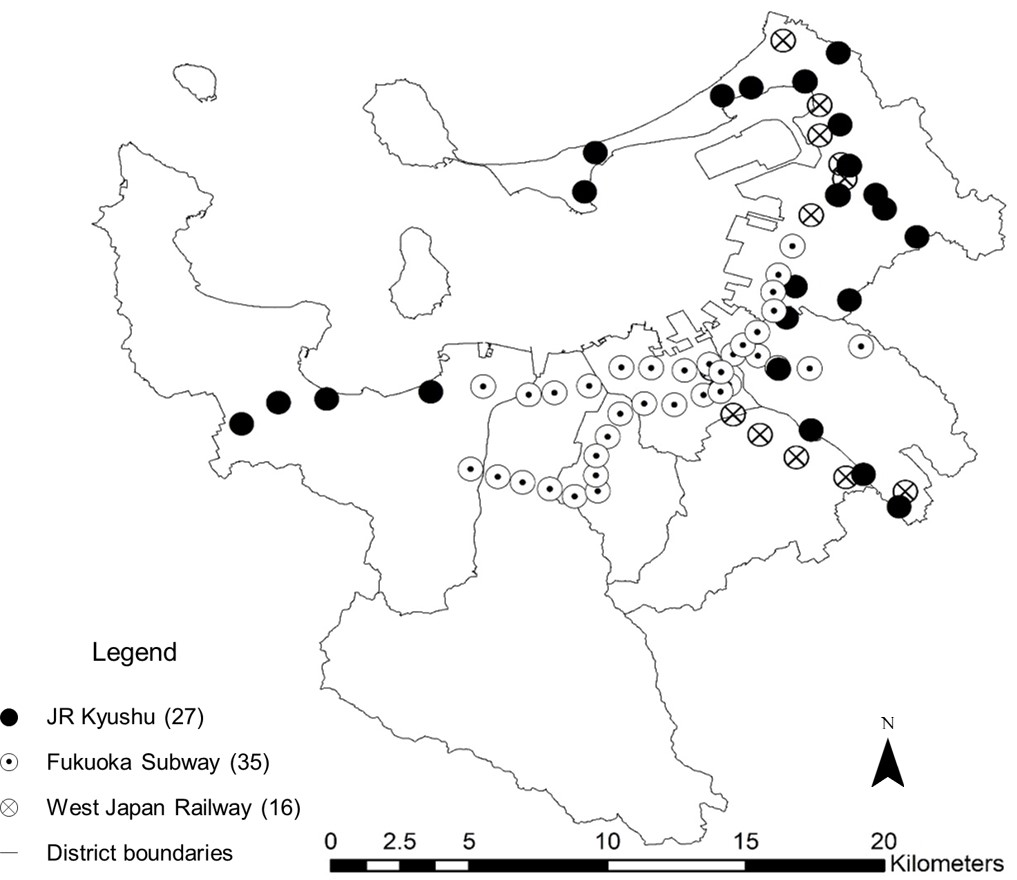
\includegraphics[width=0.8\linewidth]{chapter2/StationDistribution}
	\caption{Distribution of transit stations}
	\label{fig:chp2:StationDistribution}
\end{figure}

%
\subsection{Data preparation}
The original data covered the range of all the main cities in Northern Kyushu Area, which has 483,556 records of trip chaining behavior. The available data onto this study mainly includes trip chaining behavior and socio-demographic characteristics, as shown in the Table \ref{tab:chp2:Data}.

% Table 1
\begin{table}[htbp]
	\centering
	\caption{Available data contents}
	\label{tab:chp2:Data}
	\small
	\renewcommand{\arraystretch}{1.25} % 重设表间距
	\begin{tabular}{ll}
		\Xhline{1.5pt}
		Category                      & Feature\\
		\midrule
		\multirow{7}[0]{*}{Trip chaining behavior} 
		& Departure location \\
		& Departure time \\
		& Destination location \\
		& Arrival time \\
		& Transport modes \\
		& Time spent for each mode \\
		& Location of bus stop or rail transit station \\
		\Xhline{0.5pt}
		
		\multirow{6}[0]{*}{Socio-demographic attributes}
		& Age \\
		& Sex \\
		& Occupation \\
		& Trip purpose \\
		& Vehicle/License holding \\
		& Address \\
		\Xhline{1.5pt}
	\end{tabular}
\end{table}

%
To analyze the walking duration from departures to rail transit stations in Fukuoka, the first step is to extract the valid records of rail transit trip within the city area of Fukuoka from 483,556 records. The procedure of extracting the valid data is divided into 3 steps. Firstly, extracting all the person trip data that surveyed within the city area of Fukuoka; secondly, selecting the trip chaining behavior which contains the rail transit mode; thirdly, filtering the invalid data that with null value and abnormal value. The procedure of data cleaning is shown in Figure \ref{fig:chp2:DataCleaning}, at last the valid data set is reduced to a size of 4,254 trips.

% Figure 2
\begin{figure}[htbp]
	\centering
	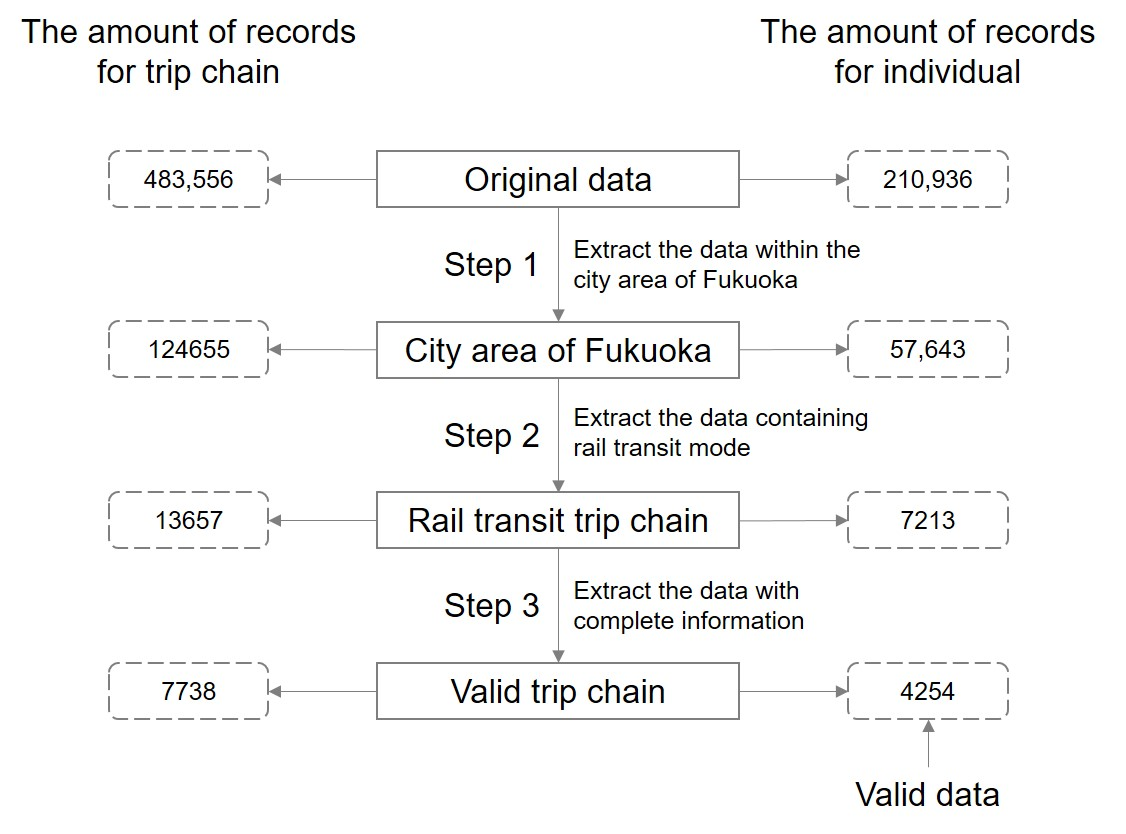
\includegraphics[width=0.9\linewidth]{chapter2/DataCleaning}
	\caption{Process of data cleaning}
	\label{fig:chp2:DataCleaning}
\end{figure}

%
Figure \ref{fig:chp2:AgeDistribution} shows the age distribution for walking trips to rail transit stations based on the finally valid data set. The passengers aged from 25 to 55 account for the majority of the whole passengers, while schoolchildren aged under 15 rarely take rail transits. The distribution graph does not show significant peak values at any specific age group. Figure \ref{fig:chp2:DurationDistribution} shows the distribution of real walking duration to stations, it has a mean value of 8.32, and the standard deviation is 4.63. Notably, there are several peak values at multiples of five. It is speculated that the peak values may be caused by deviation occurred in the investigation. Since people's feeling about the specific time or number is inaccurate, they are inclined to reply a loose answer when they are asked some questions about the details of walking duration. This inclination will count some of the real walking duration that is near to 5 multiples as the 5 multiples and finally expressed in the investigation result. Despite the bias between survey and reality, as the hypothesis H3 proposed before, passengers are viewed that they can accept the walking duration what they answered. Therefore, the peak values are considered to have no significant influence on the analysis.

% Figure 3
\begin{figure}[htbp]
	\centering
	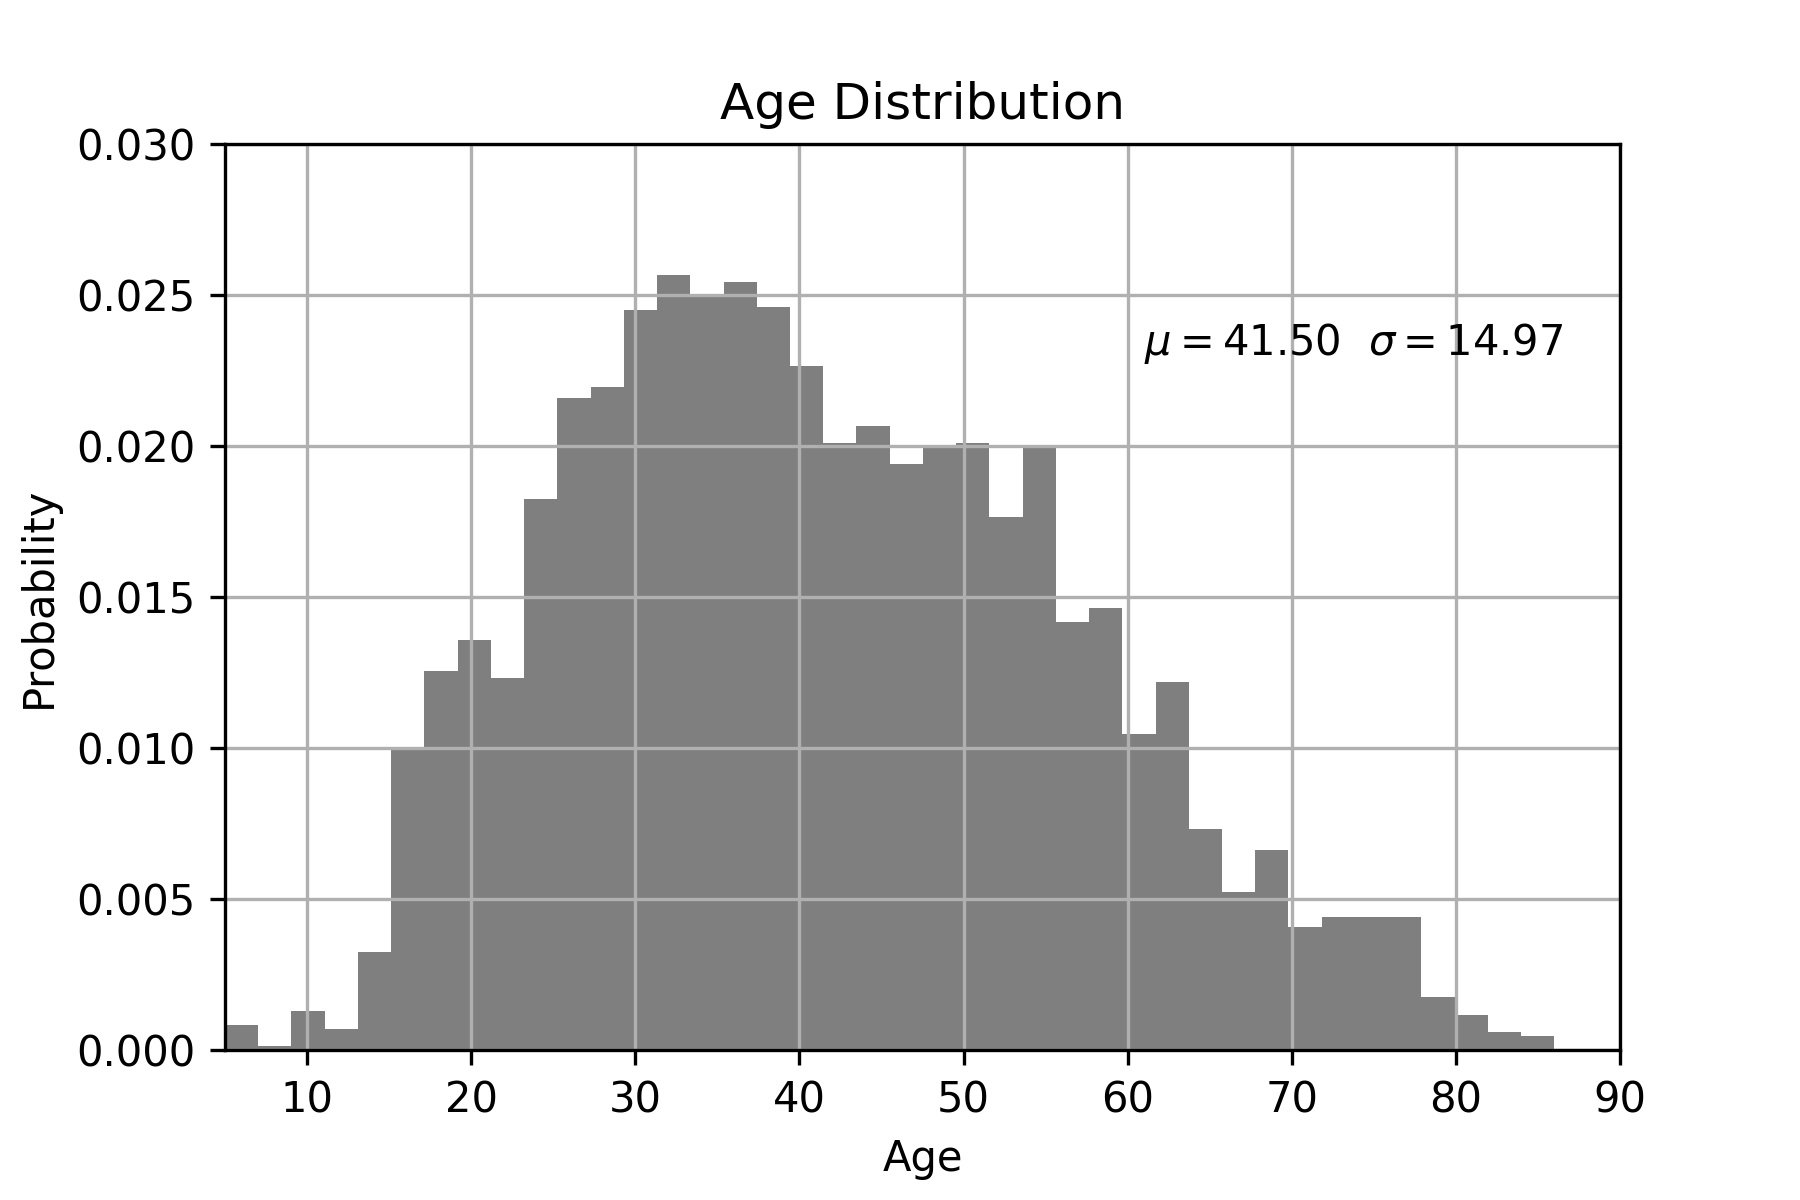
\includegraphics[width=\linewidth]{chapter2/AgeDistribution}
	\caption{Age distribution of passengers}
	\label{fig:chp2:AgeDistribution}
\end{figure}

% Figure 4
\begin{figure}[htbp]
	\centering
	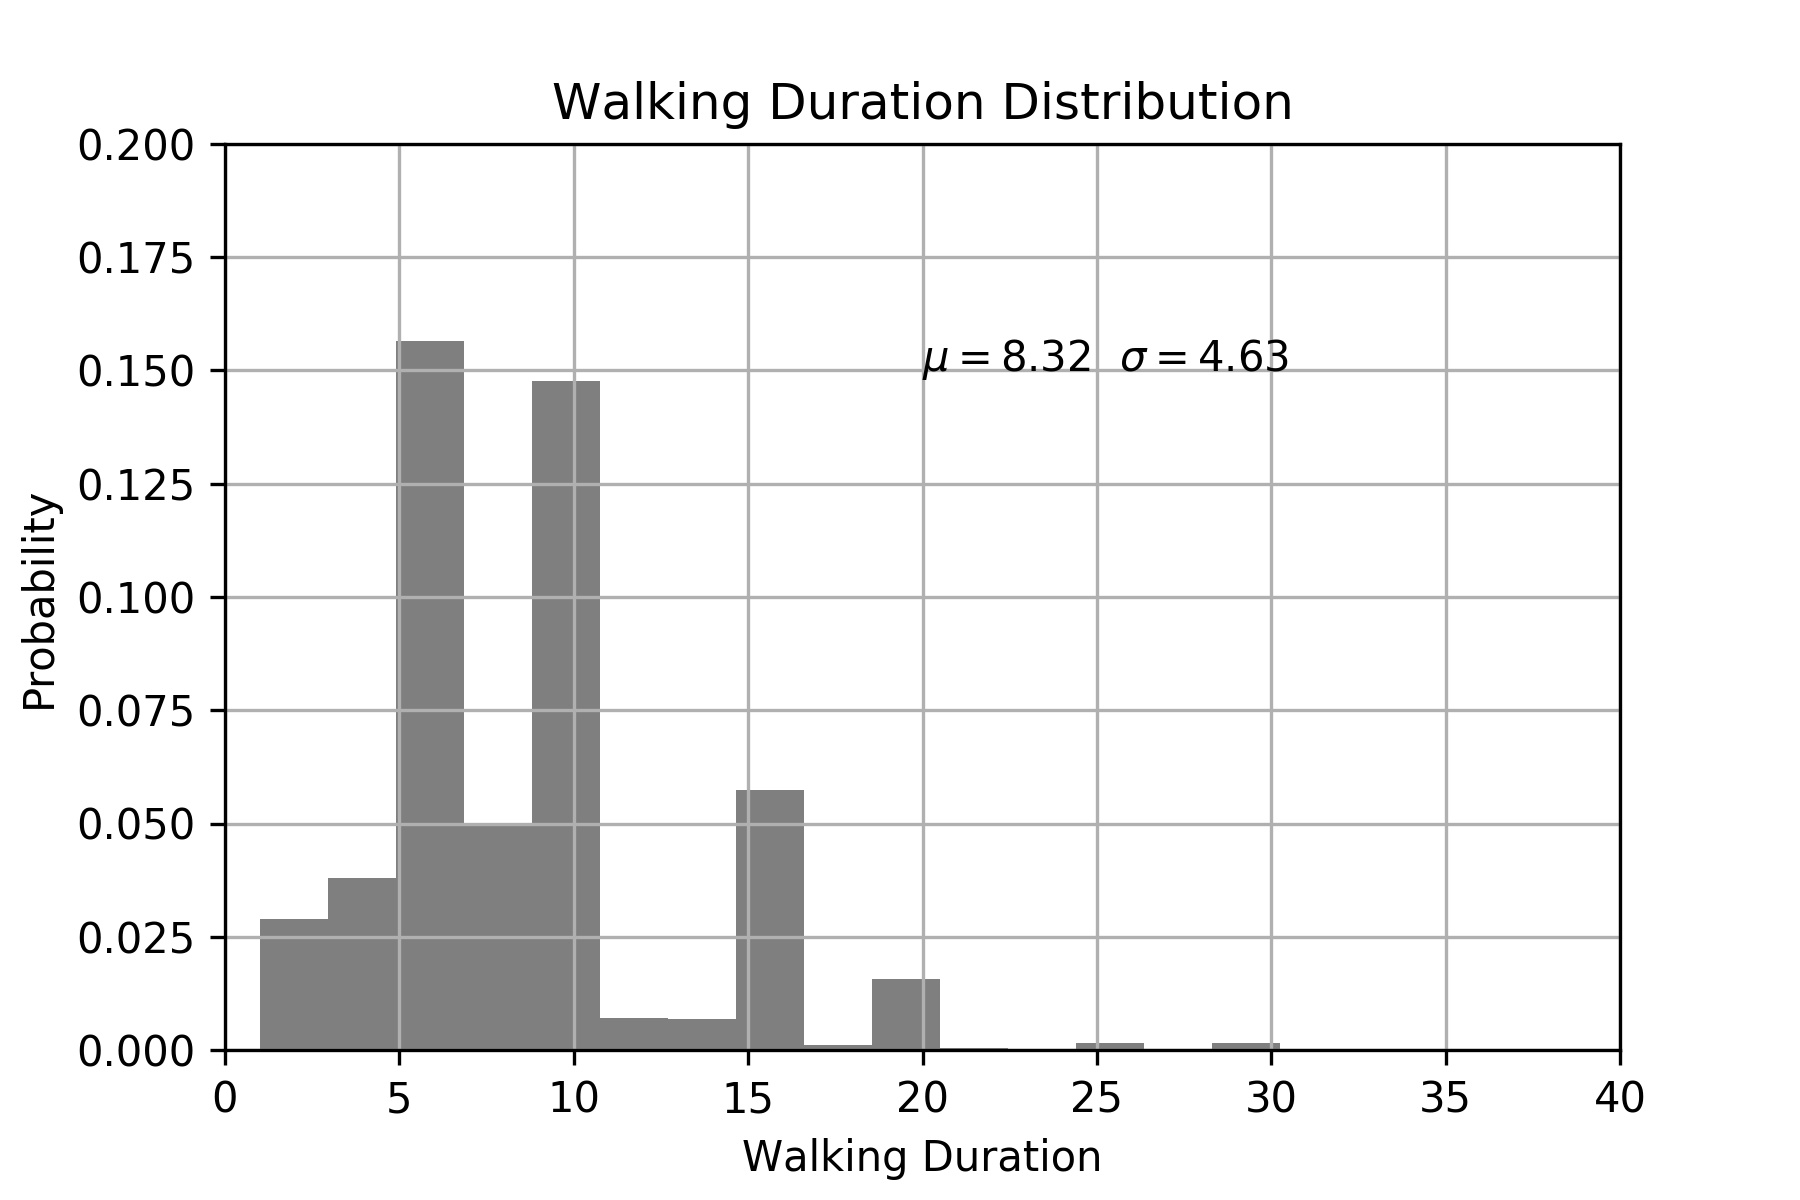
\includegraphics[width=\linewidth]{chapter2/DurationDistribution}
	\caption{Distribution of walking duration}
	\label{fig:chp2:DurationDistribution}
\end{figure}

%
\subsection{Data description}
The feature of trip purpose has 15 subcategories in the original data set, this study reclassifies them into 5 categories including commuting to work, commuting to school, official business, private purpose (such as shopping, entertainment), and going home. The feature of occupation is reclassified from 14 subcategories into 5 categories as well, they are service, technology, administration, student, and the other. Table \ref{tab:chp2:PersonAttributeStatistics} reports some of the statistical description for each feature. Overall, the average walking duration to rail transit stations is 8.32 minutes; more than 75\% of the passengers walk less than 10 minutes; most passengers walk to stations costing 5-10 minutes. In detail, there are some significant differences in the statistical description of each feature, the differences are summarized as follows.

%
\begin{itemize}
	\setlength{\parskip}{0\baselineskip} % 设置段间距
	\item People with the purpose of commuting account for the majority in the rail transit users.
	\item Most people do not accept a walking duration to transit stations more than 15 minutes.
	\item The walking duration during peak hour is longer than off-peak hour.
	\item Young and old people are inclined to spend less time on walking to rail transit stations.
	\item Passengers with the trip purposes of official business and going home tend to take shorter time for walking to rail transit stations.
	\item Passengers with the trip purpose of commuting to work are willing to accept a longer walking duration than that with other purposes significantly.
	\setlength{\parskip}{0.7\baselineskip} % 设置段间距
\end{itemize}


% Table 2
\begin{sidewaystable}[htbp]
	\caption{Statistical description of walking duration for each feature}
	\label{tab:chp2:PersonAttributeStatistics}
	\centering
	\small
	\renewcommand{\arraystretch}{1.25}
	\begin{tabular}{llrrccccccc}
		\Xhline{1.5pt}
		Features & Categories & Count & Percentage & Mean & Std & 10th & 25th & 50th & 75th & 90th\\
		
		\midrule
		& Total & 4254 & - & 8.32 & 4.63 & 3 & 5 & 8 & 10 & 15 \\
		
		\midrule
		\multirow{2}{*}{Sex}
		& Male & 2257 & 53.1\% & 8.41 & 4.63 & 3 & 5 & 8 & 10 & 15 \\
		& Female & 1996 & 46.90\% & 8.22  & 4.63 & 3 & 5 & 7 & 10 & 15 \\
		
		\midrule
		\multirow{2}{*}{Peak hour}
		& Peak & 2976 & 70.00\% & 8.51 & 4.66 & 3 & 5 & 8 & 10 & 15 \\
		& Off peak & 1277 & 30.00\% & 7.88 & 4.52 & 3 & 5 & 7 & 10 & 15 \\
		
		\midrule
		\multirow{4}{*}{Age}
		& 5-24 & 543 & 12.80\% & 8.18 & 4.7 & 3 & 5 & 7 & 10 & 15 \\
		& 25-44 & 1992 & 46.80\% & 8.36 & 4.42 & 3 & 5 & 8 & 10 & 15 \\
		& 45-64 & 1407 & 33.10\% & 8.43 & 4.83 & 3 & 5 & 8 & 10 & 15 \\
		& 65- & 311 & 7.30\% & 7.78 & 4.81 & 3 & 5 & 7 & 10 & 15 \\
		
		\midrule
		\multirow{5}{*}{Occupation}
		& Service & 1256 & 29.50\% & 8.32 & 4.57 & 3 & 5 & 8 & 10 & 15 \\
		& Tech & 721 & 17.00\% & 8.58 & 4.89 & 3 & 5 & 8 & 10 & 15 \\
		& Office & 1076 & 25.30\% & 8.44 & 4.48 & 4 & 5 & 8 & 10 & 15 \\
		& Student & 325 &  7.60\% & 8.12 & 4.73 & 3 & 5 & 7 & 10 & 15 \\
		& Null & 875 & 20.60\% & 8.03 & 4.62 & 3 & 5 & 7 & 10 & 15 \\
		
		\midrule
		\multirow{5}{*}{Purpose}		
		& Commuting to work & 2697 & 63.40\% & 8.69 & 4.51 & 4 & 5 & 9 & 10 & 15 \\
		& Commuting to school & 287 & 6.70\% & 8.19 & 4.60 & 3 & 5 & 8 & 10 & 15 \\
		& Official business & 153 & 3.60\% & 7.10 & 5.05 & 2 & 3 & 5 & 10 & 15 \\
		& Private purpose & 789 & 18.60\% & 7.82  & 4.78 & 3 & 5 & 7 & 10 & 15 \\
		& Going home & 327 & 7.70\% & 7.17 & 4.67  & 2 & 5 & 5 & 10 & 15 \\
		%
		\Xhline{1.5pt}
	\end{tabular}
\end{sidewaystable}


%
\section{Analysis}
% 流程概述:1. 方差分析识别特征值。2. 随机森林决策树拟合关系。3. 验证集进行验证结果
% 本研究
The independent variable in this study is the probability of walking the given walking duration or more. Based on the above description of the data set, several typical thresholds of walking duration are selected to explore the passenger walking preference. According to the literature, walking access to rail transit stations generally ranged from 400 meters to 1000 meters in terms of different city types, travel habits, also the needs of research purpose \cite{guerra2012half,murray1998public,o1996walking,keijer2000people,zhao2003forecasting,alshalalfah2007case}. If converting this walking distance into walking duration by using the walking speed of 4.8 km/h, the walking duration would range from 5 minutes to 13 minutes \cite{bohannon1997comfortable}. In the case of Fukuoka City, more than 40\% of the samples walk less than 5 minutes, and the walking duration less than 13 minutes covers about 85\% of the total samples. It can be inferred that the 5-minute walking duration is easy to accept, while a walking duration longer than 13 minutes is thought to be hard to accept. In addition, the average walking duration of this study is about 8 minutes, it can be considered that this median value is ambiguous to be accepted. As a result, the three representative thresholds of 5, 8, 13 minutes are picked as the typical threshold for estimating the relationship between individual attributes and walking duration. 

At each threshold of walking duration, the exploration of the walking preference in terms of passenger attributes is extended to three steps. The first step is to identify the effective features using the Analysis of Variance (ANOVA). Secondly, training the model to obtain the functional relationship between the dependent variables and the independent variable. With this trained model, inputting a new set of passenger attributes can obtain a probability of walking the given walking duration or more. Finally, inputting the test data set into this trained model to evaluate the model description ability.

%
\subsection{Effective attributes selection}

% 结果的读法
The effective features are identified using ANOVA. The feature which has the p-value less than 0.05 (this feature relevant with the dependent variable at the confidence level of 95\%) is picked out and listed in Table \ref{tab:chp2:ValidFeatures}. In the column of "Effect" in this table, the "M" means the passengers with this feature tend to walk more than the given threshold of walking duration, while the "L" is opposite that the passenger with this feature tends to walk less than the given threshold.

% Table 3
\begin{sidewaystable}[htbp]
	\caption{Valid features and the effect at each threshold}
	\label{tab:chp2:ValidFeatures}
	\centering
	\small
	\renewcommand{\arraystretch}{1.25} % 重设表间距
	
	\begin{tabular}{lrlrlr}
		\Xhline{1.5pt}
		\multicolumn{2}{c}{5 min threshold} & \multicolumn{2}{c}{8 min threshold} & \multicolumn{2}{c}{13 min threshold} \\
		
		\midrule
		Features & Effect* & Features & Effect* & Features & Effect* \\
		Age over 65 & M	& Female & L & Age 45-64 & L \\
		Peak hour & L & Age 25-44 & L & Peak hour & L \\
		O\_Null & M & Peak hour & L & P\_commuting to work & L \\
		P\_commuting to work & L & P\_commuting to work & L & P\_ private purpose & M \\
		P\_official business & M & P\_official business & M	& & \\
		P\_private purpose & M & P\_ private purpose & M & & \\
		P\_going home & M & P\_ going home & M & & \\
		\Xhline{1.5pt}
	\end{tabular}
	%
	\begin{description}
		\small
		\label{note:tab:chp2:ValidFeatures}
		\item[*Note:] The "M" means passengers with this feature tend to walk more than the given threshold of walking duration, while the "L" is opposite.
	\end{description}
\end{sidewaystable}

% 表的描述
As shown in \ref{tab:chp2:ValidFeatures}, at the threshold of 5-minute, the features of trip purposes and peak hour play the most important role in determining the willingness of walking duration. Situations are changed at the threshold of 8-minute, the importance of age and gender raised in some extent, while the features of trip purposes are not changed from that of 5-minute. The features of 13-minute show obvious differences from that of 5-minute and 8-minute. This result of feature selection is also consistent with common sense and partly confirmed by the previous research. Most of the walking duration is distributed around the average walking duration of 8 minutes, it can be considered that walking duration ranging from 5 to 13 minutes are sensitive to individual attributes. The walking duration more than 13 minutes are not accepted by most people even if they have different individual attributes. The threshold less than 5 minutes is also not sensitive to individual attributes since the 5-minute threshold is generally accepted by most passengers.

%
\subsection{Feature estimation}

% 随机森林的说明。主要是为什么使用这个模型。
This issue has been converted into a binary choice problem as stated before. The models of the decision tree, Bayesian, support vector machine (SVM), logistic regression, and neural network are widely adopted to estimate this type of problem. With the limitation of the volume of sample and features, also the unknown feature distribution, the decision tree model is considered to be a good choice because of the good generalization for different forms of data. Furthermore, to avoid the structure of the tree being too complicated, also to reduce the possibility of over-fitting of data which is easily occurred in the decision tree model, this study introduces an improved model of the decision tree, the random forest decision model, to tackle this problem. Random forest decision is an ensemble learning method mainly for classification and prediction. The random forest decision is an extension and improvement for the decision tree model, it is operated by constructing a multitude of decision trees and randomly selecting the features when training the model \cite{ho1995random,ho1998random}. 

% 随机森林的具体过程
The effective features identified by the ANOVA (Table \ref{tab:chp2:ValidFeatures}) are used in the random forest decision to estimate the probability of walking the given walking duration or more. As to the estimation, the data set is divided into two parts, 50\% of the sample are used for fitting the model thus obtaining the functional relationship, the rest 50\% are used for testing the ability of prediction. The prediction process is presented in Figure \ref{fig:chp2:RandomForests}. For the random forest decision, the prediction is not obtained from the only one decision tree but the multitude of decision trees constructed by random selection of features and samples. The dependent variable at the given threshold of walking duration to rail transit stations is calculated by equation \ref{eq:chp2:probability} based on the mean prediction.

% Figure 5
\begin{figure}[htbp]
	\centering
	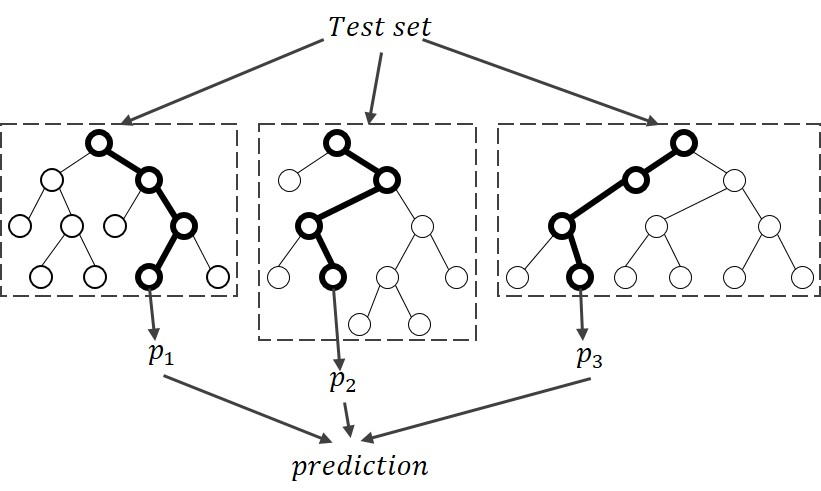
\includegraphics[width=0.7\linewidth]{chapter2/RandomForests}
	\caption{Prediction process in random forests decision}
	\label{fig:chp2:RandomForests}
	\begin{description}
		\small
		\label{note:fig:chp2:RandomForests}
		\item[Note:] The final prediction is obtained by the vote of results obtained from the same set of features in different trees
	\end{description}
\end{figure}

%
\subsection{Prediction and evaluation}
% 加入对kappa系数的叙述
The prediction is obtained from the forest random decision model, the flow is shown in Figure \ref{fig:chp2:MachineLearningFlowchart}. The accuracy of results is evaluated from the perspective of both individual and group. The summary of the prediction results is shown in Table \ref{tab:chp2:ConfusionMatrix}.

% Figure 5
\begin{figure}[htbp]
	\centering
	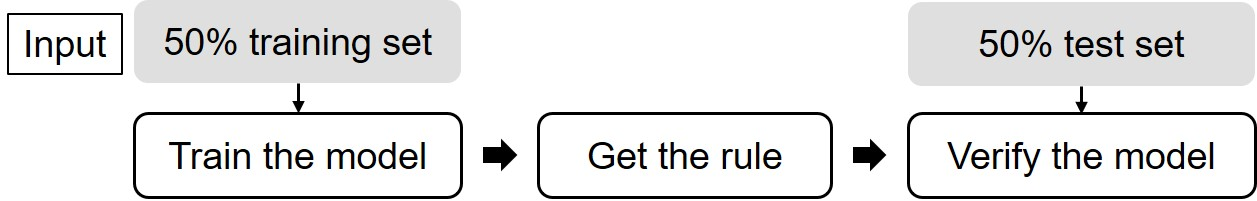
\includegraphics[width=0.7\linewidth]{chapter2/MachineLearningFlowchart}
	\caption{The flow of getting prediction from a trained model}
	\label{fig:chp2:MachineLearningFlowchart}
\end{figure}

% 混淆矩阵5分钟
\begin{table}[htbp]
	\caption{Confusion matrix of the prediction at each threshold}
	\label{tab:chp2:ConfusionMatrix}
	\centering
	\begin{tabular}{p{6em}<{\centering}p{3em}<{\centering}p{3em}<{\centering}p{3em}<{\centering}p{3em}<{\centering}}
		\Xhline{1.5pt}
		& & \multicolumn{2}{c}{Prediction} & \\ 
		\midrule
		& & \multicolumn{1}{c}{0} & \multicolumn{1}{c}{1} & Total \\
		\multirow{2}{6em}{\centering{5-minute \\ test data set}} & 0 & 394  & 494 & 888 \\
		& 1 & 377 & 862 & 1239 \\
		& Total & 771 & 1356 & 2127 \\ 
		
		\midrule
		& & \multicolumn{1}{c}{0} & \multicolumn{1}{c}{1} & Total \\
		\multirow{2}{6em}{\centering{8-minute \\ test data set}} & 0 & 699  & 442 & 1141 \\
		& 1 & 588 & 398 & 986 \\
		& Total & 1287 & 840 & 2127 \\
		
		\midrule
		& & \multicolumn{1}{c}{0} & \multicolumn{1}{c}{1} & Total \\
		\multirow{2}{6em}{\centering{13-minute \\ test data set}} & 0 & 1404  & 399 & 1803 \\
		& 1 & 229 & 95 & 324 \\
		& Total & 1633 & 494 & 2127\\ 
		\Xhline{1.5pt}
	\end{tabular}
\end{table}

%
The prediction for individuals is evaluated by Cohen's kappa coefficient ($K$). Cohen's kappa coefficient is a statistic which measures inter-rater agreement for categorical items. It is generally thought to be a more robust measure than simple percent agreement calculation, as $K$ takes into account the possibility of the agreement occurring by chance. Based on the confusion matrix of the prediction result, the Cohen's kappa coefficients of each the walking duration threshold 5, 8, 13 minutes are calculated as shown in Table \ref{tab:chp2:Evaluation}. Magnitude guidelines are also put forward in the literature. Perhaps the first was Landis and Koch \cite{landis1977measurement}, who characterized values $< 0$ as indicating no agreement and $0 – 0.20$ as slight, $0.21 – 0.40$ as fair, $0.41 – 0.60$ as moderate, $0.61 – 0.80$ as substantial, and $0.81 – 1 $as almost perfect agreement. 

The prediction for groups is expressed by using using the method of simple moving average, and is evaluated by the coefficient of determination ($R^2$). Figure \ref{fig:chp2:Prediction} is the comparison between the trend lines of test data set and prediction. The trend line of the surveyed values based on the test data set is calculated by the mean probability of a group people that have close predicted values. The trend line is drawn by a descending order for predicted values. From the comparison of predicted values and surveyed values, the coefficients of determinations at each threshold are obtained. As is shown in Table \ref{tab:chp2:Evaluation} the prediction at the threshold of 5 minutes is better than that at the threshold of 8 and 13 minutes, which has a $R^2$ of 0.843. The prediction for the 13-minute is slightly good for a $R^2$ of 0.426, while it is not so good for the case of 8 minutes ($R^2$ is 0.221). 

According to the evaluation, if checking the prediction for individuals, the accuracy of this model is still not enough to explain the individual behavior. But the trend line of group prediction infers that this result can reflect the behavior of people with specific individual attributes at a given threshold of walking duration. 

% Trend line
\begin{figure}[htbp]
	\centering
	\begin{minipage}{0.49\linewidth}
		\centering
		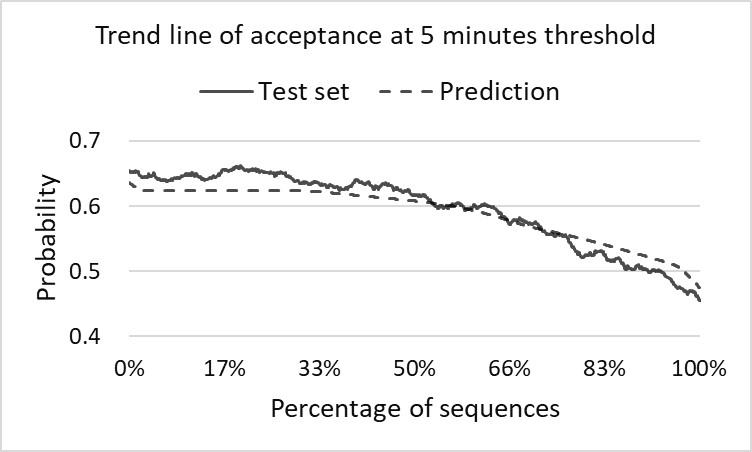
\includegraphics[width=\linewidth]{chapter2/Prediction5Min} \\
		\centering{5-minute}
		\label{note:tab:chp2:Prediction5}
	\end{minipage}
	\hfill % 横向填充,均匀分布
	\begin{minipage}{0.49\linewidth}
		\centering
		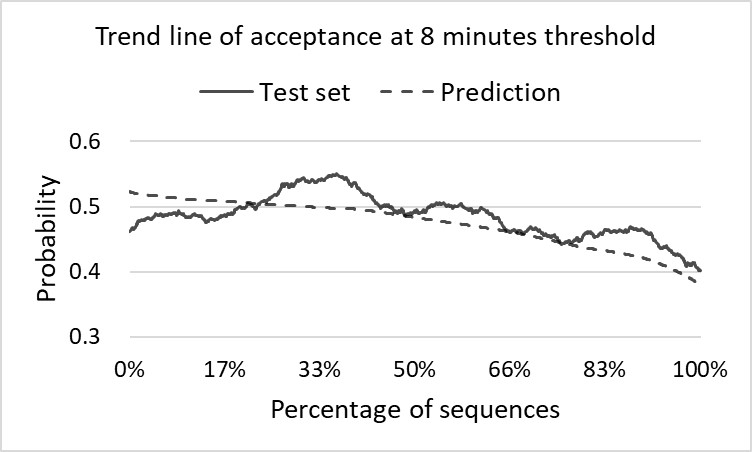
\includegraphics[width=\linewidth]{chapter2/Prediction8Min} \\
		\centering{8-minute}
		\label{note:tab:chp2:Prediction8}
	\end{minipage}
	
	\vfill % 纵向填充,均匀分布
	\begin{minipage}{0.49\linewidth}
		\centering
		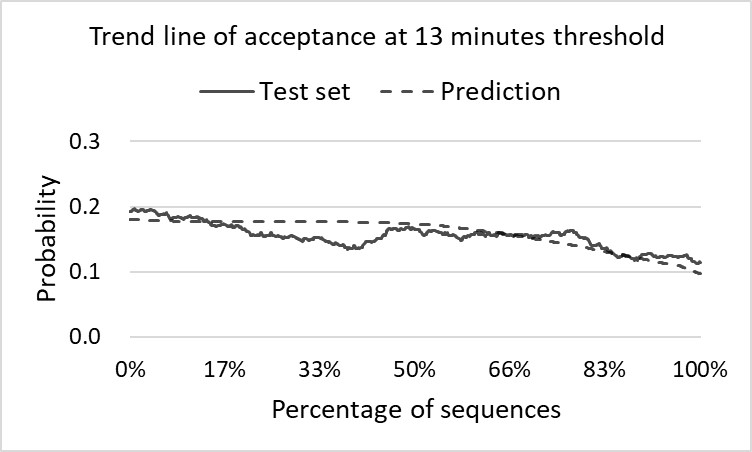
\includegraphics[width=\linewidth]{chapter2/Prediction13Min} \\
		\centering{13-minute}
		\label{note:tab:chp2:Prediction13}
	\end{minipage}

	\caption{Trend line of prediction and test set}
	\label{fig:chp2:Prediction}
\end{figure}

% Evaluation
\begin{table}[htbp]
	\caption{Evaluation of the prediction}
	\label{tab:chp2:Evaluation}
	\centering
	\begin{tabular}{rrrr}
		\Xhline{1.5pt}
		& \multicolumn{1}{c}{5-minute} & \multicolumn{1}{c}{8-minute} & \multicolumn{1}{c}{13-minute} \\
		\midrule
		\multicolumn{1}{c}{Kappa index} 						 & 0.142 & 0.016 & 0.060 \\
		\multicolumn{1}{c}{Coefficient of determination}  & 0.843 & 0.221 & 0.426 \\
		\Xhline{1.5pt}
	\end{tabular}
\end{table}

%
\section{Discussion and conclusion}
% 结论部分首先照抄PPT部分,详细说明每个时间节点。然后说明预测和评价

This study described and analyzed 4254 records of rail transit trip. Three thresholds of walking duration are examined. From the result shown in Table \ref{tab:chp2:ValidFeatures}, trip purpose is the most important factor of determining the walking duration at all the 3 thresholds. The feature of peak hour is also significant in explaining the walking duration. People tend to walk a longer time to stations at peak hours, while people with private purpose or on the way going home is not willing to choose a stations far away. For the details of each threshold, the unemployed people and the elderly people tend to walk less than 5 minutes to stations; people whose age is between 25 and 44 are unwilling to walk more than 8 minutes; people aged from 45 to 64 can accept walking more than 13 minutes to stations more easily.

%
However, summarized above is only the description of the distribution of walking duration in terms of each feature which is hard to apply. In fact, the data onto this study is obtained from a factual investigation but not a willingness survey. Once people have made a decision on walking to rail transit stations, the walking duration is just representation of the location of departures and the walking speed. It is hard to say whether the individual attributes affected the walking duration, maybe due to this reasons few existing studies can explain the relation between walking duration and individual attributes quantitatively correctly. Under the hypothesis proposed before, the distribution of walking duration can be viewed as a reflection of the acceptability of walking duration, which should have relationship to people's individual attributes. According to hypothesis 3, the behavior that a passenger chose to walk to a station means this passenger can accept the walking duration from the departure to that station. Based on the hypothesis H1 and H2, if the people that accepted the given threshold of walking duration shows significant differences in individual attributes, it means they have a different acceptability of walking duration to the others.

%
As explained above, this study examined the differences in individual attributes of passengers that accepted the given thresholds of walking duration. As the results, people with different individual attributes shows different acceptability at each threshold of walking duration. According to the evaluation from the method of simple moving average, the model of 5-minute threshold has a better explanatory ability, the model of 13-minute threshold is a little weaker, and the model of 8-minute threshold is not good. Here are some possible reasons for explaining the results. The selected thresholds of walking duration 5, 8, 13 minutes represent the lower boundary, the mean value, and the upper boundary of the main distribution of walking duration respectively. Since the commonly acceptable walking duration ranges from 5 to 13 minutes, it can be inferred that the passengers having different preference to walking duration may have significant features. However, as the mean value of walking duration, it can be thought that most of the walking duration are distributed around 8 minutes, for passengers there may be some randomness in making the decision of whether walking to rail transit stations. For the other threshold values near the mean value of 8 minutes, it also can be inferred that people may have some ambiguity in choosing whether to walk to stations or not. This explanation can also be confirmed by the result of valid features selection. There are 5 identical features of both 5-minute and 8-minute threshold, which means people with those features are not sensitive to the threshold from 5 to 8 minutes.

%
The results of the random forest decision showed some predictive power for groups of people, especially at the threshold of 5 minutes. However, it did not give available prediction on individual predictions, which means the application of this study needs a certain number of sample scale, there is still a lot of work need to be done on improving the accuracy of prediction. In the next stage of this research, we plan to apply the results to predict the willingness of a group of people at a specific walking duration. By using this prediction, for example, if knowing the individual characteristics of residents in a particular area locating from the rail transit station $T$ minutes, the general acceptability of walking to the station for the residents in this area should be predictive. Therefore, this prediction of willingness is expected to be used in planning the catchment area of rail transit stations or estimating the catchment area of existing stations.

% reference
\clearpage % 新起一页
\bibliographystyle{apacite}
% \bibliographystyle{IEEEtran}
\bibliography{ref}